% -*- Mode:TeX -*-

\documentclass[twoside,titlepage,12pt]{article}
\usepackage{fancyhdr}
\usepackage[margin=1in]{geometry}
\usepackage{hyperref}
\usepackage{enumerate}
\usepackage{enumitem}
\usepackage{graphicx}
\usepackage[nottoc,notlot,notlof]{tocbibind}
\usepackage{amsmath}
\usepackage{listings}
\usepackage{color}
\usepackage[T1]{fontenc}
\usepackage{float}
\usepackage{subcaption}
\usepackage[utf8]{inputenc}
\usepackage{amsfonts}
\usepackage{verbatim}

\author{Edward Lee}
\title{Mesh Creation for Finite Element Methods}

\numberwithin{equation}{section}

\geometry{
  headheight = 3ex,       % <-- and this
	 headsep = 2ex,          % <-- and this
}
\pagestyle{fancy}

\lstdefinestyle{fortranStyle}{
	language=[90]Fortran,
	keywordstyle=\color{red},
	commentstyle=\color{green},
	morecomment=[l]{!\ },
	numbersep=10pt,
	tabsize=4,
	showspaces=false,
	showstringspaces=false,
	basicstyle=\ttfamily\small
}

\begin{document}
\maketitle

\tableofcontents
\newpage

\begin{comment}
\part{Thanks}

I thank Helene Barucq, for accepting me into this research group, encouraging me to "tutoyer le monde," and organizing workshops for the group. She is truly a welcoming and friendly personality.

I thank Conrad Hillairet for the time he has spent on helping me through the fortran code, and the whole Hou10ni project in general. Lover of biscuits and wines, Conrad has been my invaluable guide in the team.

I thank Simon Ettouati for the invaluable explanations he has given me on the Elasticus project. 

I thank Julien Diaz for the logistical work he went through to make sure that my stay in Pau went well.

I thank the entire team at Magique 3D for their friendly and welcoming attitude, their patience with my mediocre French, good humor, especially Florian, Lionel, Hendrik, Ha, Vincent, Mamadou, Victor, Izar, Aralar, and Clia.
\end{comment}


\begin{comment}
\part{Preface}

After my first year of my Bachelors degree in Theoretical Mathematics at Massachusetts Institute of Technology, I chose an internship in applied mathematics in the context of petroleum seismic imaging. During the 2 months while I was at this internship, I gained a significant amount of knowledge, in both domains of geophysics and mathematics. Specifically, I learned the concepts behind various methods for solving Helmholtz equations acoustic and elastic wave equations by using Finite Element Methods, Finite Difference Methods, Discontinuous Galerkin Methods. Solving these equations by resolving 2D meshes allows one to simulate the propagation of waves in arbitrary media. This in turn facilitates methods such as Full-Waveform-Inversion, Kirchoff Migration, Reverse Time Migration. In the case of Reverse Time Migration, waves and inverse waves are used to calculate reflection coefficients in the media, in turn generating an image of the underground. However, the applications of this method extend beyond the petroleum industry. For example, by solving the Maxwell Equations, it is possible through subtle variations of the methods to generate an image of the suns subsurface, which is actually another project here at Magique3D.
\end{comment}


% \newpage
\section{INRIA}

The Institut National de Recherche en Informatique et Automatique is a public establishment dedicated to technological research and software development. INRIA's goal is to create a network of talent both french and international concerning its five fields of research: http://www.inria.fr/en/research/research-fields/five-fields-of-research. 

\subsection{History}

C/P'ed from: \href{http://www.inria.fr/en/institute/inria-in-brief/history-of-inria}{History of INRIA}

The creation of IRIA, the precursor of INRIA, along with a number of other organisations, was a symbol of the proactive policies to develop cutting-edge technologies and the means to produce them. This prompted the country to create a national champion in the form of the CII (the Compagnie Internationale pour l'Informatique) in December 1966, following the takeover of Bull by General Electric. The creation of IRIA was also a response to a desire to develop an institute that was close to industry and capable of educating the country in the fields of computer science and control.


1967 was the year of the Plan Calcul, a French governmental programme aimed at promoting a national computer manufacturing industry and associated research activities. This programme included the creation of a new government body responsible for computer science, the Délégation à l'informatique, and a new research institute, IRIA, under the leadership of Michel Laudet. IRIA was a new kind of organisation, close to the private sector, which prefigured a new relationship between the public sector and industry. It was designed to be the active arm of the CII.


As soon as it was created, IRIA began to organise international conferences, inviting big names from the fields of computer science and applied mathematics. The institute rapidly earned itself an international reputation. One of its priorities was training: summer schools were set up with EDF and the CEA, as well as a training centre: the centre for practical studies in computer science and control (CEPIA), which delivered 5,000 hours of classes in its first year alone.


In 1973, André Danzin organised IRIA around SESORI (the department for the consolidation and orientation of computer science research, led by Michel Monpetit, which was responsible for links with the Plan Calcul) and Laboria (the computer science and control research laboratory) with Jacques-Louis Lions. Laboria was organised around research projects, with its own resources, objectives, project managers and schedules. But with only 80 researchers, Laboria was nowhere near big enough.


The period from 1974 to 1979 saw both a maturing of the institute and a few missed opportunities. Under the leadership of Jacques-Louis Lions, Laboria built itself a strong identity. Under the presidency of Valéry Giscard d'Estaing, the European collaborations came under threat, while a lack of flexibility and resources prevented the institute from making quick progress. There was real dissemination of knowledge, the institute developed a reputation in other countries, long-term strategies were established, and IRIA began to push towards Rennes and think about Sophia Antipolis. But in the late seventies it was still struggling to find its place.


SESORI launched a number of pilot projects to produce products that could be used in industry. One example was its computer-aided design and drawing mission (MICADO), which made it possible to coordinate research in CAD. SESORI was responsible for coordinating national work on various themes ranging from robotics to breakdown prevention, from shape recognition to digital image processing.



At Laboria, the Cyclades project explored innovative solutions for creating a computer network based on the Cigale packet switching data network. Presentations in France, Europe and the United States put IRIA at the forefront of the world scene in this field. Despite this, the project was suspended in 1976. The Spartacus project, a collaboration with Inserm (the French National Institute for Health and Medical Research), the CNRS (the French National Centre for Scientific Research) and the CEA (the French Atomic Energy Commission), aimed to develop a system allowing tetraplegics to regain some independence.

In 1979, decentralisation threatened IRIA's existence: there was talk of relocation to Sophia Antipolis or a merger with IRISA in Rennes (which had been created with IRIA's help in 1975). Eventually, Jacques-Louis Lions was able to keep the institute at Rocquencourt, and an 'N' was added to its name. In accordance with the Decree of 27 December 1979, the institute would henceforth be known as Inria.


The appointment of Jacques-Louis Lions as Inria Chairman in 1980 marked a turning point. In the 1980s, the institute, still with very limited resources, developed a model centred around the excellence of its research, with the constant aim of ensuring technology transfer to industry (creation of innovative businesses in strategic sectors). Inria created a network for European researchers (ERCIM, European Research Consortium for Informatics and Mathematics ) and played a major role in the development of the Internet in Europe. After a lot of trial and error, Inria now had clear aims and a strong international reputation.


As part of a process of decentralisation and regional development, the National Institute for Research in Computer Science and Control built centres all over the country:

Irisa and then the Rennes research unit from 1975;
the Sophia-Antipolis research unit in 1983;
the Lorraine research unit / Loria in 1986;
the Rhône-Alpes research unit in 1992;
the Futurs research unit from 2003, incubating 3 future units in Bordeaux, Lille and Saclay.
20 years of business creation

Inria's innovative technology transfer activities included the filing of patents, agreements with industrial partners, the running of Consortia, and support for innovative businesses. Between 1984 and 2004, 80 businesses were created, 45 of which still exist. The number of international collaborations grew rapidly.


4-year strategic plans, corresponding to 4-year contracts with the State, committed Inria to a number of priorities and performance objectives in terms of research, innovation and technology transfer on a global scale.
The first strategic plan (1994-1998) focussed on four research themes: networks and systems, software engineering and symbolic computing, human-machine interaction, images, data and knowledge, and simulation and optimisation of complex systems.


Futurs batiments INRIA Bordeaux Sud-Ouest
After celebrating its fortieth anniversary in 2007, Inria continues to expand. Between 1999 and 2009, its workforce doubled . Three new research centres in Saclay, Bordeaux and Lille were added to the 5 existing centres in Rocquencourt,  Rennes,  Sophia Antipolis, Nancy and  Grenoble. Firmly rooted in local industrial and academic ecosystems, Inria is pursuing an increasing involvement in the European Research Area. With a resolutely international outlook, it is contributing to the global profile of computational sciences. Convinced that the future of our societies lies in digital technology, Inria is tackling research subjects crucial to the social issues of today.

Inria is helping to bolster the competitiveness of the economy in a sector that creates a large number of jobs. Its policy of partnerships with industry and SMEs illustrates its proactive approach to technology transfer.

In order to disseminate scientific information and knowledge more effectively, Inria is committed to open access and sharing of data. The Institute is also involved in the field of freeware.

Furthermore, it is one of the founder members of the Alliance des sciences et technologies du numérique (ALLISTENE), the aim of which is to eliminate barriers between research players and develop partnership initiatives.


More than half of Inria project-teams are involved in the European Framework Programmes for Research and Development (FPRD). The European Commission ranks Inria in the top ten contributing organisations. As part of FPRD 7, Inria has helped to identify two major scientific challenges: the Internet of the future and the digital patient. In 2006, Inria signed up to the European Charter for Researchers.


The strategic plan for 2008-2012 sets out the scientific objectives for the immediate future, based on the challenges of the 21st century. Inria is strengthening and diversifying its partnerships with other scientific disciplines and the business world (strategic partnerships), in France and in Europe, in the USA and with emerging countries (China, India, South America, Africa).

\subsection{Organization}

Click here: \href{http://www.inria.fr/en/institute/organisation}{Organization of INRIA}

% 
\newpage
\section{Research within INRIA}

\subsection{Five Fields of Research}

Within INRIA, there are five essential fields of research. Within each field, there are smaller subfields with project-teams dedicated to topics within those subfields. Listed here are all five fields of research and the subfields that are listed at the Bordeaux Sud-Ouest Center of Research.
\begin{enumerate}

\item \href{http://www.inria.fr/en/research/research-fields/five-fields-of-research/applied-mathematics-computation-and-simulation}{Applied Mathematics, Computation and Simulation}

\subitem Numerical schemes and simulations
\subitem Stochastic approaches
\subitem Optimization, machine learning and statistical methods

\item \href{http://www.inria.fr/en/research/research-fields/five-fields-of-research/algorithmics-programming-software-and-architecture}{Algorithmics, Programming, Software and Architecture}

\subitem Algorithmics, Computer Algebra and Cryptology
\subitem Embedded and Real-time Systems

\item \href{http://www.inria.fr/en/research/research-fields/five-fields-of-research/networks-systems-and-services-distributed-computing}{Networks, systems and services, distributed computing}

\subitem Distributed and High Performance Computing
\subitem Distributed programming and Software Engineering

\item \href{http://www.inria.fr/en/research/research-fields/five-fields-of-research/perception-cognition-interaction}{Perception, Cognition \& Interaction}

\subitem Interaction and visualization
\subitem Robotics and Smart environments

\item \href{http://www.inria.fr/en/research/research-fields/five-fields-of-research/digital-health-biology-and-earth}{Digital Health, Biology and Earth}

\subitem Earth, Environmental and Energy Sciences
\subitem Modeling and Control for Life Sciences
\subitem Computational Biology
\subitem Computational Neuroscience and Medicine

\end{enumerate}


\subsection{Centers of Research}

\begin{enumerate}
\item \href{http://www.inria.fr/centre/bordeaux}{Bordeaux - Sud-Ouest}
\item \href{http://www.inria.fr/centre/grenoble}{Grenoble - Rhone-Alpes}
\item \href{http://www.inria.fr/centre/lille}{Lille - Nord Europe}
\item \href{http://www.inria.fr/centre/nancy}{Nancy - Grand Est}
\item \href{http://www.inria.fr/centre/paris-rocquencourt}{Paris - Rocquencourt}
\item \href{http://www.inria.fr/centre/rennes}{Rennes - Bretagne Atlantique}
\item \href{http://www.inria.fr/centre/saclay}{Saclay - Ile-de-France}
\item \href{http://www.inria.fr/centre/sophia}{Sophia Antipolis - Mediterranee}
\end{enumerate}

\subsection{Project Teams}
CP'ed from \href{http://www.inria.fr/en/research/research-teams/project-team-model}{Inria Project-team Model}

Ever since it first began, Inria has made use of an original research model founded on a basic entity:the project-team. This model is the component that structures the institute's research activities. Made up of around 20 individuals, the project-team is formed around a "scientific leader", who defines scientific objectives on a topic approved by the institute.


\subsection{Magique 3D}

C/P'ed from: \href{https://team.inria.fr/magique3d/research/}{magique3D/research}

\subsubsection{Purpose and Research Themes}
    Magique-3D is a joint project-team between Inria and the Department of Applied Mathematics (LMA) of the University of Pau in partnership with CNRS. The mission of Magique-3D is to develop and validate efficient solution methodologies for solving complex three-dimensional geophysical problems, with a particular emphasis on problems arising in seismic imaging, in response to the local industrial and community needs. Indeed, as it is well known, the region of Pau has long-standing tradition in the Geosciences activities. However, in spite of the recent significant advances in algorithmic considerations as well as in computing platforms, the solution of most real-world problems in this field remains intractable. Hence, there is a scientific need of pressing importance to design new numerical methods for solving efficiently and accurately wave propagation problems defined in strongly heterogeneous domains.


The research record of Magique-3D group covers a large spectrum of accomplishments in the field of wave propagation including (a) the design, validation, and performance assessment of a class of DG-methods for solving efficiently high frequency wave problems, (b) the construction, convergence analysis, and performance assessment of various absorbing-type boundary conditions that are key ingredients for solving problems in infinite domains, and (c) the development of asymptotic models that are the primary candidate in the presence of heterogeneities that are small compared to the wave length.

    Magique-3D has built strong collaborations and partnerships with various institutions including (a) local industry (TOTAL), (b) national research centers (ONERA and CEA), and (c) international academic partnerships (e.g. Interdisciplinary Research Institute for the Sciences (IRIS) at California State University, Northridge, USA; University of Pays Basque at Bilbao, Spain; University of Novosibirsk, Russia).

\subsubsection{Mathematical modeling of wave propagation}

    The development of migration software with preserved amplitudes is of great interest for imaging geological structures based on the propagation of seismic waves. Most of the geophysicists use the Kirchhoff formalism with a posteriori corrections of the amplitude. Magique-3D proposes instead to evaluate the exact amplitude directly by developing more complete modeling techniques. This implies the construction of new models and the analysis of their qualitative and numerical properties. New models must incorporate absorbing conditions in order to be able to compute the solution in bounded domains. The construction of such conditions is optimized in order to improve the accuracy of the numerical solution and/or reduce the computational cost.
    

\subsubsection{Numerical simulation, parallel computing, GRID computing}

    The spectral element method (SEM) has recently shown its efficiency for the computation of synthetic seismograms compared to more classical approaches such as finite difference schemes. Magique-3D uses the SEM to quantify the effects of both topography and variations of geological structures on the propagation of seismic waves. Magique-3D also considers simplified inverse problems for 3D structures, which makes it possible for instance to analyze the propagation of surface waves in weathered zones in the context of active seismic experiments performed by the petroleum industry. Magique-3D also intends to develop a finite element method optimized to run on a parallel computer for the study of geomorphology. This project could in part be done jointly with Scalapplix. Magique-3D also intends to study the propagation of elastic waves in fractured media by coupling quasi-analytic methods near the fractures with a finite element method in the surrounding medium. The numerical methods involved in this work all result in a high computational cost, and we therefore want to benefit from recent technological advances by developing algorithms that can not only run on very large parallel computers but also on so-called "grids" of computers ("GRID computing").


\newpage
\section{Context: Hydrocarbon Exploration}

The processes of Reverse Time Migration and solving forward problems in creating images of the underground is primarily used in the field of hydrocarbon exploration. Petroleum geologists and geophysicists looking for petroleum or natural gas underground utilize these tools to help 

\subsection{Seismic Acquisition}

\subsection{Method of Exploration: Seismic Reflection}

\subsection{Processing the data}

\subsection{Seismic Waves}
\subsubsection{Waves in 3D}

\newpage
\section{Presentation of the Problem}

The problem that we are trying to solve is the simulation of the propagation of waves. In this section, we present the problem in the context of seismic imaging, an essential component of the seismic processing. We explain its importance in various migration methods, as well as how as a forward problem, numerical simulation is also essential to its counterpart, the inverse problem.

\subsection{Inverse Problem: Seismic Imaging}

Part of the data processing is seismic imaging, whose goal is to produce an accurate image of the underground that geophysicists can interpret to determine the location of hydrocarbon reservoirs. Given the data, a series of pressure or velocity observations by receivers at the surface or at the seafloor, is it possible to reconstruct this image? Since we know the observations as well as one of the inputs (the source signal), and we are looking for the other inputs (the reflection coefficients), seismic imaging is thus an inverse problem whose solution is a collection of parameters we cannot directly observe. As an inverse problem in a physical setting, it is also an ill-posed problem, where we do not have enough information to get a unique solution. However, we may add new pieces of information such as well log data to the system in order to generate a more accurate image. 


One of the methods to solve the inverse problem and create the seismic image is to use Wavefield Extrapolation Migrations, a technique that uses the full wavefield as opposed to ray theory \cite{EAGE}. This class of migration methods includes the recently popular method called Reverse Time Migration or RTM for short, and can be very computationally expensive, requiring up to hundreds or even thousands of cores. The essence of the calculations here lies in the calculation of the reflection coefficient at every point using the back-propagated upgoing wavefield $P_{up}(x,y,z,t)$ (from the receiver) as well as downgoing wavefield $P_{d}(x,y,z,t)$. Under ideal circumstances, the reflection coefficient $r$ is equal to $\frac{P_{up}(x,y,z,t)}{P_d(x,y,z,t)}$ for all time steps $t$. However, circumstances are never ideal and it is a better idea to use the correlation coefficient calculation:

$$r = \frac{\sum\limits_t P_{up}(x,y,z,t) P_d(x,y,z,t)}{\sum\limits_t P_d^2(x,y,z,t) + \epsilon}$$ 

where $\epsilon$ is a small constant to prevent possible division by $0$, and we use summation instead of integration over time because we are using a computer and numerical algorithm.



\subsection{Forward Problem: Simulation of Wave Propagation}

An important part of solving this inverse problem is computing the solution to the forward problem. Since we need to know the values of the upgoing and downgoing wavefield at each time step (the pressure or velocity measurements at every point in the simulated earth), In essence, solving the forward problem, also known as solving the wave equations (or Maxwell's equations in the context of electromagnetism), is the simpler job of numerical simulation of the propagation of waves - the essence of this paper. 


\subsection{Acoustic Wave Equation}

The reason it is also known as solving the wave equation is that we frequently work with domains that are overly complex than the simple one-dimensional uniform case in university Differential Equations courses. The wave equation is simply a partial differential equation that describes the pressure in the domain. In this paper, we work with the simplest wave equation - the acoustic wave equation - and solve it in the time domain as a demonstration of concept:

$$\nabla u(x,t) - \frac{1}{c(x)^2} \frac{\partial^2 u(x,t)}{\partial t^2} = f(x,t)$$

where $u(x,t)$ is the pressure, dependent on space and time, $c(x)$ is the wave propagation velocity, dependent on space, and $f(x,t)$ is the source signal.


For a complex domain with regions of different physical characteristics, it becomes necessary to simulate the solutions numerically in order to visualize the changes in pressure. We give here examples of the solutions that the Hou10ni and Elasticus programs at Inria Magique3D produce, in the frequency and time domain in Figures \ref{fig:Water-Frequency},\ref{fig:Water-Time}: 

\begin{figure}[ht]
	\centering
	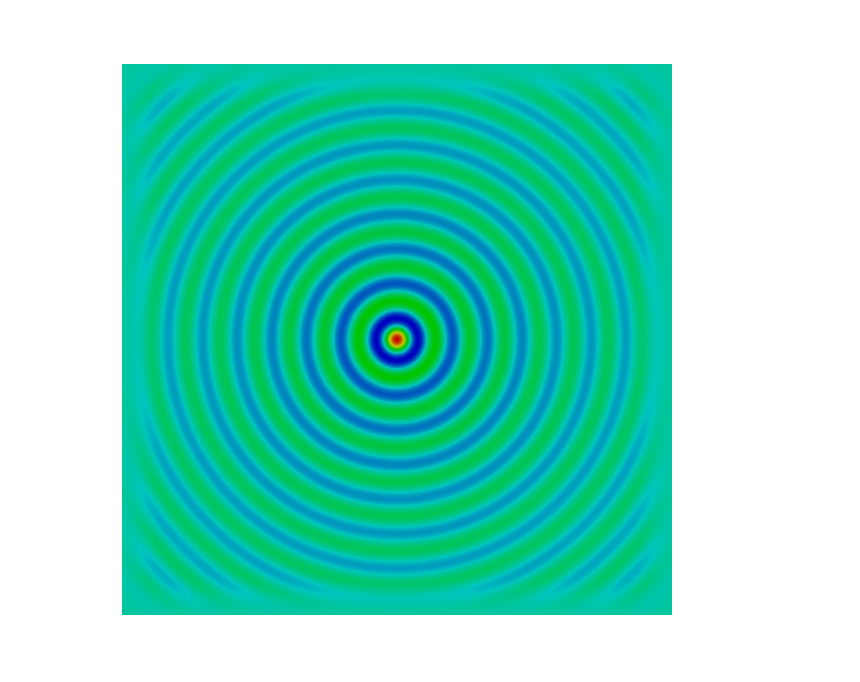
\includegraphics[width=0.7\textwidth]{Images/Water-Frequency.png}
	\caption{Solution to Acoustic Wave Equation in Frequency Domain by Hou10ni program}
	\label{fig:Water-Frequency}
\end{figure}


\begin{figure}
	\centering
	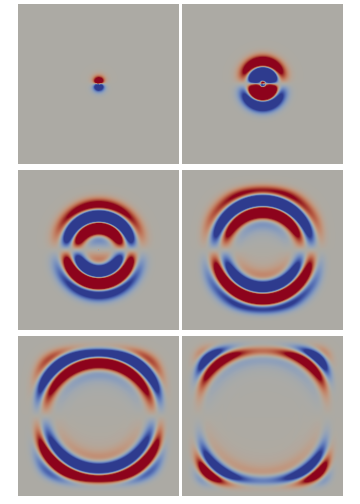
\includegraphics[width=0.9\textwidth]{Images/time.png}
	\caption{Solution to Elastic Wave Equation in Time Domain by Elasticus program}
	\label{fig:Water-Time}
\end{figure}


\subsection{Infinite Domains: Perfectly Matched Layers}

It is also necessary for computational purposes, to limit the size of the computational domain. Although in physical reality, the domain is infinite as the wavefield generated by the source propagates outward, it is necessary to introduce a limit. These limits are currently classified into two major types - Absorbing Boundary Conditions (ABC's) and Perfectly Matched Layers (PML's). Absorbing Boundary Conditions, while more stable in more circumstances than Perfectly Matched Layers, are frequently less effective in mitigating waves incident upon the boundary. For this paper, we use PML, which are easier to implement.

\subsection{Numerical Methods: Discontinuous Galerkin}

There are many numerical methods being used to solve differential equations today, frequently in the domain of structural analysis, including Finite Difference Method (FDM), Finite Element Method (FEM), Finite Volume Method (FVM), and finally Discontinuous Galerkin Methods (DG). The core of these methods lies at the calculation of the desired variable at many points in the domain, frequently using a mesh, whether structured or unstructured, to do so. There exist methods to calculate variables at fluidly changing coordinates without the use of a mesh, notably Smoothed Particle Hydrodynamics, but currently most applications do not use these methods. 

While today, the most popular is FEM for its flexibility in creating meshes that fit well to arbitrary domains, we use the method of Discontinuous Galerkin for this paper.




%\subsubsection{Anisotropy}

%\subsubsection{Elasticity Tensor C}



% \newpage
\section{Discontinuous Galerkin Method}

The Discontinuous Galerkin Method is a method of resolving differential equations through a mesh. It is similar to the Finite Element Method and the Finite Volume Method. This section is for the reader with a beginner's understanding of the Finite Element Method.

\subsection{Basic Overview}


\begin{figure}[ht]
\centering
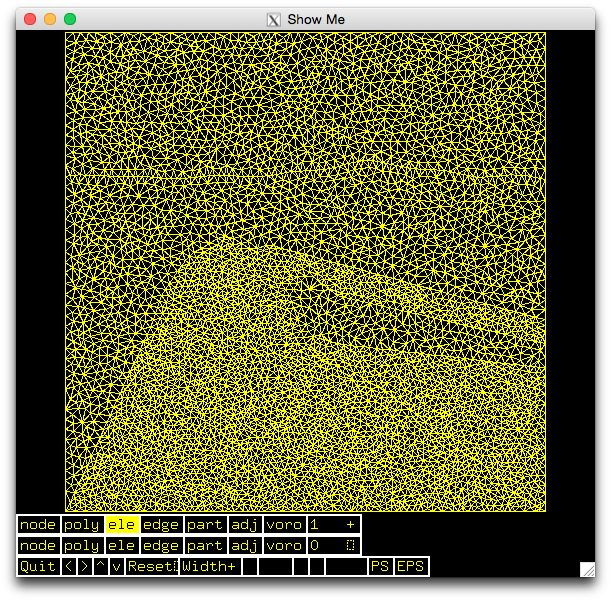
\includegraphics[width=0.7\textwidth]{Images/Example-Mesh.png}
\caption{Example Mesh used to cover example data}
\label{fig:couches5-mesh}
\end{figure}

"Solving differential equations" (such as the acoustic wave equation) is a term that is commonly thrown around without much attention to the essential components in numerical analysis. For the common case, it means: \textbf{given a domain} (for example $[0,10]$ in one dimension or the unit sphere in three dimensions), we \textbf{take a mesh} (set of segments, triangles, tetrahedrons, etc) that covers the domain, and find the values of the variable we are solving for at \textbf{certain moments in time} and at \textbf{certain points in the domain} that are determined by the mesh.

The Discontinuous Galerkin Method is a method to "solve differential equations". It can be considered a combination of Finite Element Methods (Continuous Galerkin) and Finite Volume Methods. In other words, Discontinuous Galerkin methods are finite element methods that use discontinuous basis functions, thus acquiring more robustness for discontinuous processes. Because the base function polynomials are discontinuous and do not extend over a large stencil,the  Discontinuous Galerkin Method is easily parallelized, and the Mass Matrix is able to be inverted by blocks. Like the Finite Volume Methods, Discontinuous Galerkin methods calculate surface integrals and fluxes of discontinuous terms.

\subsection{Basis Functions}

In Discontinuous Galerkin Methods, we can raise the accuracy of our solution by increasing the order of the polynomials that approximate it. 

The way we represent our solution to the differential equation, is a group of polynomials for each element in the mesh; each polynomial takes a value of $1$ at a certain point called a node, and $0$ at all the other nodes defined in the element. Each base function is discontinuous in that it can take nonzero values inside its own element, but takes the value $0$ on other elements. This is the reason the method is called Discontinuous Galerkin and also the fundamental reason it is easily parallelizable. We can thus define the solution as the linear combination of those functions:

$$u(x,t) = \sum\limits_{i=1}^n c_i(t)\phi_i(x)$$ 
where $c_i(t)$ is merely a time-dependent coefficient and $\phi_i(x)$ is the space-dependent base function defined solely on its corresponding element.


But an important observation that helps us significantly speed up the computation is realizing that we can perform all our integrals on a simple reference element, and then map it onto the actual element. Refer to Figure ~\ref{fig:Reference-Elements} for the visual definition of the reference element in 2 and 3 dimensions as well as the transformation mapping. Here we let the use of the hat in $\hat{E}$ represent the reference element, and the lack of use represent the actual element.


\begin{figure}[ht]
	\centering
	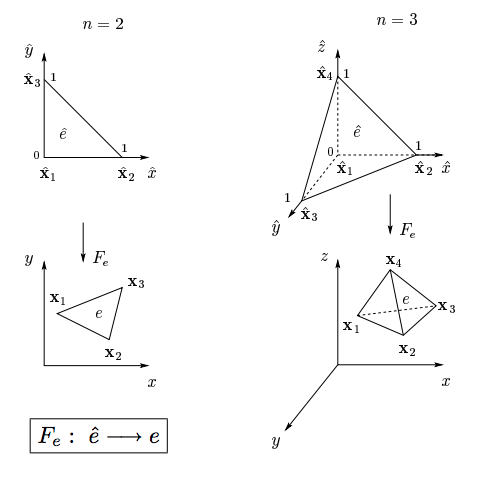
\includegraphics[width=0.7\textwidth]{Images/Reference-Elements.png}
	\caption{Reference Elements transformed to the actual Elements}
	\label{fig:Reference-Elements}
\end{figure}


Given an order $p$, the specific nodes on the reference element are defined as:

$$(\hat{x_i}, \hat{y_j}, \hat{z_k}) = \left( \frac{i}{p}, \frac{j}{p}, \frac{k}{p} \right) \text{ for each } (i,j,k) \in \mathbb{N}^3 \mid i + j + k \leq p$$ 

and we represent the $l$'th node location as $x_l$.

In order to calculate the base functions for the arbitrary order $p$, we can use linear algebra. Namely, we wish to find the base function polynomials of the form:

$$\sum\limits_{i+j+k \leq p} C_{i,j,k} x^i y^j z^k = \sum\limits_{j=1}^n C_j m_j(x)$$
where we have $n$ nodes, $n$ polynomials, and $n$ monomials per polynomial. 

Because the $i$'th polynomial takes a value of $1$ at the $i$'th node and $0$ at all the others, we can represent this relationship with a matrix equation, where the vector on the right is the $i$'th unit vector:

$$\begin{bmatrix}
m_1(x_1) & m_2(x_1) & \ldots & m_n(x_1) \\
m_1(x_2) & m_2(x_2) & \ldots & m_n(x_2)\\
m_1(x_3) & m_2(x_3) & \ldots & m_n(x_3) \\
\ldots   & \ldots   & \ldots & \ldots \\
m_1(x_n) & m_2(x_n) & \ldots & m_n(x_n) 
\end{bmatrix} 
\begin{bmatrix}
C_1 \\
C_2 \\
C_3 \\
\ldots \\
C_n
\end{bmatrix}
= \begin{bmatrix}
0 \\
\ldots \\
1 \\
\ldots \\
0
\end{bmatrix} $$

We can find the polynomial by computing the values of $C_j$,
and summing their product with their corresponding monomials. For simplicity, represent the equation as $S \boldsymbol{C} = \boldsymbol{I}$. By multiplying both sides by $S^{-1}$, we have that $\boldsymbol{C}$ is equal to the $i$'th column of of $S^{-1}$. Thus, we have our $i$'th base function polynomial.

\subsection{Variational / Weak Formulation (is that what it's called?)}

In order to begin analyzing the acoustic wave equation, we multiply the equation by a test function $v(x,t)$. Do not worry too much about the purpose of the test function, a short summary is that without it, there is no guarantee of finding a function that satisfies the equation. Then we integrate over each element $E$:

\begin{equation} 
\int_E \nabla \cdot \nabla u(x,t) v(x,t) dV + \int_E \frac{\partial^2 u(x,t)}{\partial t^2} v(x,t) dV = \int_E f(x,t) v(x,t) dV 
\end{equation}

Frequently, we need to decompose the integral of the laplacian operator $\nabla \cdot \nabla$ on the domain of the element into an integral on the domain of the element's boundary face in order to place Absorbing Boundary Conditions (new set of differential equations) on the boundary face. In order to do that, we apply Green's first identity to obtain:

\begin{equation}
\int_{\Gamma_E} c^2 v(x,t) \nabla u(x,t) \cdot dS - \int_E c^2 \nabla u(x,t) \cdot \nabla v(x,t) dV - \int_E \frac{\partial^2 u(x,t)}{\partial t^2} v(x,t) dV = \int_E f(x,t) v(x,t) dV
\label{eq:Variational-Form}
\end{equation}

where $\Gamma_E$ is the faces of the element $E$.

\subsection{Mass, Stiffness, Damping Matrices}

We desire to rewrite Equation ~\ref{eq:Variational-Form} in terms of matrices. Specifically, we wish to write it as:

\begin{equation}
\mathcal{M} \frac{\partial^2}{\partial t^2} U_h + c \mathcal{B} \frac{\partial}{\partial t} U_h + c^2 \mathcal{K} U_h = -\mathcal{F}
\label{eq:Matrix-Form}
\end{equation}


The Mass Matrix $\mathcal{M}$ is defined as the matrix in front of the $\frac{\partial^2}{\partial t^2}$ term. The Damping Matrix $\mathcal{B}$ is defined as the matrix in front of the $\frac{\partial}{\partial t}$ term. The Stiffness Matrix $\mathcal{K}$ is defined as the matrix in front of the term with no $t$ at all.

In order to accomplish this, we rewrite $u(x,t)$ as its discontinuous space-dependent parts and time dependent parts:
\begin{equation}
$u(x,t) = c_1(t) \phi_1(x) + c_2(t) \phi_2(x) + \ldots + c_n(t) \phi_n(x)$
\end{equation}

With this method, we can then transform the equations into a linear matrix form. For example, take the term:

\begin{equation}
\int_E \frac{\partial^2 u(x,t)}{\partial t^2} v(x,t) dV
\end{equation}

We want the equalities to be satisfied for any $v(x,t)$ in our function space, so we just need to make sure that the equalities are satisfied for $v(x,t) = \phi_i(x)$ for all $i$. We can do this by using vector and matrix operations to represent multiple equations.

\begin{equation}
\begin{bmatrix}
\int u(x,t) \phi_1 dV \\
\int u(x,t) \phi_2 dV \\
\ldots \\
\int u(x,t) \phi_n dV
\end{bmatrix}
\end{equation}

\begin{equation}
= \begin{bmatrix}
\int \phi_1 \sum\limits_{i=1}^n \frac{\partial^2 c_i(t)}{\partial t^2} \phi_i dV \\
\int \phi_2 \sum\limits_{i=1}^n \frac{\partial^2 c_i(t)}{\partial t^2} \phi_i dV \\
\ldots \\
\int \phi_n \sum\limits_{i=1}^n \frac{\partial^2 c_i(t)}{\partial t^2} \phi_i dV
\end{bmatrix}
\end{equation}

\begin{equation}
= \begin{bmatrix}
\sum\limits_{i=1}^n \frac{\partial^2 c_i(t)}{\partial t^2} \int \phi_i \phi_1 dV \\
\sum\limits_{i=1}^n \frac{\partial^2 c_i(t)}{\partial t^2} \int \phi_i \phi_2 dV \\
\ldots \\
\sum\limits_{i=1}^n \frac{\partial^2 c_i(t)}{\partial t^2} \int \phi_i \phi_n dV
\end{bmatrix}
\end{equation}

\begin{equation}
\label{eq:Stiff-Mat}
= \begin{bmatrix}
\int \phi_1 \phi_1 dV & \int \phi_1 \phi_2 dV & \ldots & \int \phi_1 \phi_n dV \\
\int \phi_2 \phi_1 dV & \int \phi_2 \phi_2 dV & \ldots & \int \phi_2 \phi_n dV \\
\ldots                & \ldots                & \ldots & \ldots \\
\int \phi_n \phi_1 dV & \int \phi_n \phi_2 dV & \ldots & \int \phi_n \phi_n dV \\
\end{bmatrix} 
\frac{\partial^2}{\partial t^2} 
\begin{bmatrix}
c_1(t) \\
c_2(t) \\
\ldots \\
c_n(t)
\end{bmatrix}
\end{equation}

\begin{equation}
\label{eq:Stiff-Var}
= M \frac{\partial^2}{\partial t^2} U_h
\end{equation}

where $M$ is the Mass matrix and $U_h$ is the vector of coefficients defining $u(x,t)$. This is possible for all of the matrices, and we will investigate further.

\subsection{Transformation}

Because we are calculating the terms on the reference element $\hat{E}$ and not on the actual element $E$, we need to be able to map our obtained reference values to actual values. But first, it is necessary to define the linear transformation of the coordinates in terms of matrices and vectors. 

Once again, we reference Figure ~\ref{fig:Reference-Elements} for the definition of $\boldsymbol{\hat{x_1}}, \boldsymbol{\hat{x_2}}, \boldsymbol{\hat{x_3}}, \boldsymbol{\hat{x_4}}, \boldsymbol{x_1}, \boldsymbol{x_2}, \boldsymbol{x_3}, \boldsymbol{x_4}$. Then we have the relation:

\begin{equation}
F_E(\hat{x}, \hat{y}, \hat{z}) = A \begin{bmatrix}
\hat{x} \\ 
\hat{y} \\ 
\hat{z}
\end{bmatrix} + \boldsymbol{b}
= \begin{bmatrix}
x_2-x_1 & x_3-x_1 & x_4-x_1 \\
y_2-y_1 & y_3-y_1 & y_4-y_1 \\
z_2-z_1 & z_3-z_1 & z_4-z_1
\end{bmatrix} \begin{bmatrix}
\hat{x} \\
\hat{y} \\
\hat{z}
\end{bmatrix} + \begin{bmatrix}
x_1 \\
y_1 \\
z_1
\end{bmatrix}
\end{equation}

which we can see as a stretching of the reference element and then translation from $\boldsymbol{\hat{x}}$ to $\boldsymbol{x}$.

Now, when we are changing variables in integrals to determine those integrals on the actual elements, we know that the Jacobian is $|\det A|$



\subsection{Mass Matrix Calculation}
The value of the Mass Matrix $\mathcal{M}$ is given by Equation ~\ref{eq:Stiff-Mat} and ~\ref{eq:Stiff-Var}, and the entry at $(i,j)$ is calculated by:

\begin{equation}
$\int_{\hat{E}} \phi_i \phi_j dV$
\end{equation}

which is a simple job of integrating multivariate polynomials and can be done by utilizing 3rd party libraries such as SymPy, or by self-coding a polynomial integration system.
 
\subsection{Damping Matrix Calculation}

When using Perfectly Matched Layers, it is no longer necessary to decompose the laplacian to produce a boundary integral. Therefore, we do not have a term with the first derivative of time $\frac{\partial}{\partial t}$, and we do not have a Damping Matrix $\mathcal{A}$.

\subsection{Stiffness Matrix Calculation}

The value of the Stiffness Matrix $\mathcal{B}$ is given by.

\subsection{RHS Calculation}

The term $\mathcal{F}$ on the right hand side (RHS) is:
\begin{equation}
\begin{bmatrix}
\int f(x,t) \phi_1(x,t) dV \\
\int f(x,t) \phi_2(x,t) dV \\
\ldots \\
\int f(x,t) \phi_n(x,t) dV
\end{bmatrix}
\end{equation}

Given the source function $f(x,t)$, typically a Gaussian distribution multiplied by a Dirac delta function, the integrals in the vector $\mathcal{F}$ are fairly simple to calculate at any given time step. Only the entries in $\mathcal{F}$ that correspond to the element that contains the point source $f(x,t)$ will have integrals that evaluate to non-zero values.

\subsection{Time Steps}

Up until now, we have been working out the details of determining the values of $u(x,t)$ in space. Now we work out how to simulate the progression of those values in time. In order to do so, we must use Finite Differences to transform the time derivatives of $u(x,t)$ into more appealing terms using $u(x,t_i)$, the value of $u$ at certain time steps. 

\begin{equation}
\frac{\partial^2}{\partial t^2} u(x,t) \approx \frac{u(x,t+\delta t) - 2 u(x,t) + u(x,t-\delta t)}{\delta t^2}
\end{equation}

\begin{equation}
\frac{\partial}{\partial t} u(x,t) \approx \frac{u(x,t+\delta t) - u(x,t-\delta t)}{\delta t}
\end{equation}




And we are done :)















\newpage
\section{Mesh Creation} \label{Mesh-Creation}

In order to solve the wave equation in arbitrary media, both acoustic and elastic, it is necessary to create a mesh of elements, also known as simplexes, that allows the computation to be split into a collection of smaller and simpler computations on each element; the smaller solutions can then be collected into the overall solution given those arbitrary media. Here we use third party programs to split the domain into meshes of triangles and tetrahedrons. 

\subsection{Format of the .poly file}

The format of the .poly file is different in the Triangle (two dimensional) and TetGen (three dimensional) softwares. 

\subsubsection{Triangle \cite{TrianglePoly}}

Click here: \href{https://www.cs.cmu.edu/~quake/triangle.poly.html}{Triangle .poly file format} 


One line: <\# of vertices> <dimension (2)> <\# of attributes> <\# of boundary markers (0 or 1)>

Following lines: <vertex \#> <x> <y> [attributes] [boundary marker]

One line: <\# of segments> <\# of boundary markers (0 or 1)>

Following lines: <segment \#> <endpoint> <endpoint> [boundary marker]

One line: <\# of holes>

Following lines: <hole \#> <x> <y>

Optional line: <\# of regional attributes and/or area constraints>

Optional following lines: <region \#> <x> <y> <attribute> <maximum area>


\subsubsection{TetGen \cite{TetGenPoly}}

Click here: \href{http://wias-berlin.de/software/tetgen/fformats.poly.html}{TetGen .poly file format}

Part 1 - node list

    One line: <\# of points> <dimension (3)> <\# of attributes> <\# of boundary markers (0 or 1)>
    
    Remaining lines list \# of points:
    
    <point \#> <x> <y> <z>[attributes] [boundary marker]
    ... 

Part 2 - facet list

    One line: <\# of facets> <boundary markers (0 or 1)>
    
    Following lines list \# of facets:
    
    <facet \#>
    ... 

where each <facet \#> has the following format:

    One line: <\# of polygons> [\# of holes] [boundary marker]
    
    Following lines list \# of polygons:
    
    <\# of corners> <corner 1> <corner 2> ... <corner \#>
    
    ...
    
    Following lines list \# of holes:
    
    <hole \#> <x> <y> <z>
    
    ... 

Part 3 - hole list

    One line: <\# of holes>
    
    Following lines list \# of holes:
    
    <hole \#> <x> <y> <z>
    
    ... 

Part 4 - region attributes list

    One line: <\# of region>
    
    Following lines list \# of region attributes:
    
    <region \#> <x> <y> <z><region number><region attribute>

\subsection{Formulation of the problem}

\begin{figure}[H]
\centering
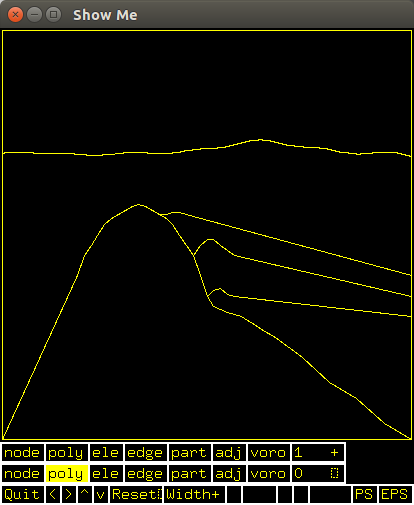
\includegraphics[width=0.5\textwidth]{Images/Original-Couches5.png}
\caption{This is the original picture of the hypothetical salt dome underneath the water and sand}
\label{fig:originalCouches5}
\end{figure}

The problem in 2 dimensions is, given the original points, how can we define an arbitrary interface between the water and the wet sand layer? In order to allow Absorbing Boundary Conditions to be effective, new points with negative coordinates were added to the image. How can we apply an affine transformation to the points so that the new image has arbitrary dimensions $(X,Y)$ and lies within the frame $[(0,0),(X,Y)]$? 

In order to extend the mesh creation to 3 dimensions, the problem of defining an arbitrary interface remains, as well as being able to apply an arbitrary dip / slope in the Y direction. 



\subsection{2 Dimensions}

In two dimensions, assuming that the original .poly file into its corresponding vertices, edges, and regions (assuming there are no holes) has been successfully parsed, the first problem is applying the affine transformation to the points. This consists of 3 steps:

\begin{enumerate}
\item Take the minimum and maximum of the X and Y coordinates: $(x_1, y_1), (x_2, y_2)$.
\item Translate the set of points so that $(x_1,y_1) \rightarrow (0,0)$ by subtracting $(x_1,y_1)$ from each point.
\item Dilate the set of points to the desired $[(0,0),(X,Y)]$ frame so that $(x_2 - x_1, y_2 - y_1) \rightarrow (X,Y)$ by multiplying each point's coordinates $x,y$ with the new dimensions $X,Y$ divided by the old dimensions $x_2 - x_1, y_2 - y_1$.
\end{enumerate}

The second problem is creating the arbitrary interface between the water and the wet sand. We represent the interface in this case as a function for example $\sin(x)$, between two endpoints for example $(0, 6\pi)$, with an amplitude for example $100$ in an image of size $3000$ along the Y-axis. Because we can only work with a finite number of points, we choose a number of steps in the X direction for example $10$. This consists of 3 steps:

\begin{enumerate}
\item Determine the two original endpoints of the interface as well as the height after the affine transform. This step can be done during the parsing stage.
\item Find the values of the function at each step in the X direction while transforming the values to have the desired amplitude at the original height: $(x,y) \rightarrow (x, \text{originalHeight} + (y)( \text{desiredAmplitude}) / (\text{maxY} - \text{minY})$
\item Add the corresponding edges between each step. Replace the original endpoints with the new endpoints.
\end{enumerate}

\subsection{3 Dimensions}




In 3 dimensions, we represent the interface as a function of $x$ and $y$ for example $\sin(x-y) \sin(x+y)$, between two endpoints in the XY plane $[(x_1,y_1),(x_2,y_2)]$, with an arbitrary amplitude. Again, we choose a number of steps in the X direction, but we must choose a number of steps in the Y direction as well. Generating the interface in 3 dimensions is quite similar to the task in 2 dimensions, so we will skip the explanation.

We now need a new function to represent the slope of the salt dome in the Y direction. Take a sequence $d$ of values all $\leq 1$. We may generate this by taking the values of a function at certain points. At each step in the Y direction, we take the corresponding value and transform the set of points representing the salt dome so that $(x,y,z) \rightarrow (x,y',z * d_i)$.

Because we extend to 3 dimensions, the edges in the Triangle .poly file extend to planes, or facets (to use the vocabulary from the TetGen documentation). The problem is then generating the facets. This can be decomposed into two subproblems: generating the facets between each Y-step, and generating the facets on the initial and last face (more difficult step). Look at Figure ~\ref{fig:facets} for clarification.

Generating the facets between each Y-step consists of two steps:
\begin{enumerate}
\item Loop over each edge, represented as $(u,v)$ where $u,v$ are vertices. Let $(u',v')$ be the corresponding points in the next Y iteration.
\item Create the facet $(u, v, v', u')$. The order is important, because the polygon must be represented in clockwise or counterclockwise order.
\end{enumerate}

Generating the facets on the initial and last face is a little more difficult and requires polygonizing the various regions in 2 dimensions. 
\begin{enumerate}
\item For each region, choose two points $q,p$ on the boundary of the region such that the interior of the region is on the left of the vector $\vec{qp}$. 
\item We proceed in the direction of $q \rightarrow p$ by taking all neighbors of $p$, excluding $q$. There should be either 1 or 2.
\item If there is only one neighbor $n$. Update $p'=n$ and $q'=p$. If there are two neighbors $a,b$, choose the neighbor $a$ such that the counterclockwise angle from $q$ to $a$ with $p$ as the origin is less than the counterclockwise angle from $q$ to $b$. Observe Figure ~\ref{fig:originalCouches5} to see that this will give you the correct neighbor.
\end{enumerate}



\begin{figure}[H]
\centering
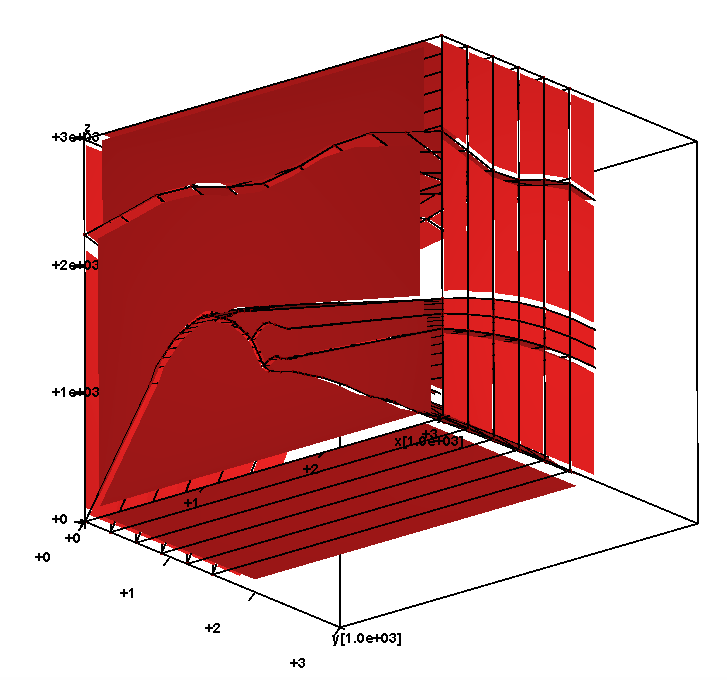
\includegraphics[width=0.7\textwidth]{Images/Facets.png}
\caption{Facets on initial face, Facets between faces, Slope of salt dome}
\label{fig:facets}
\end{figure}


\subsection{Mesh Elements}

Given the .poly file, we are able to call either triangle in 2 dimensions or tetgen in 3 dimensions to create the .mesh, .ele, etc files containing all the elements and their information. 

In 2 dimensions we call:
\begin{center}
\textbf{triangle -pqneAa file.poly}
\end{center}


In 3 dimensions we call:
\begin{center}
\centering{\textbf{tetgen -pqneAa file.poly}}
\end{center}

And we get the files, viewable by either the Showme program that comes with Triangle software, or the Tetview program that comes separately from Tetgen. Here is Figure ~\ref{fig:Elements} displaying the 3-dimensional mesh elements:

\begin{figure}[ht]
	\centering
	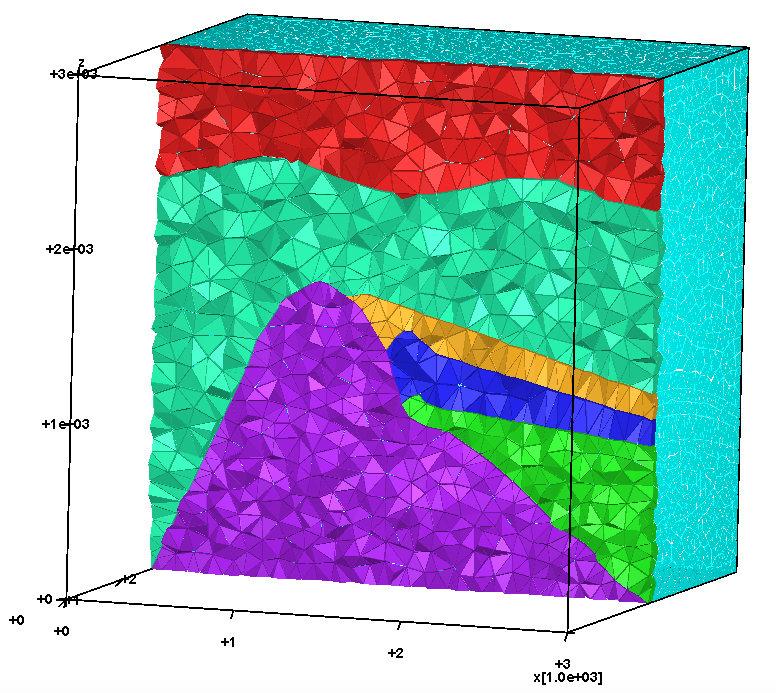
\includegraphics[width=0.7\textwidth]{Images/Elements.png}
	\caption{Elements in 3 Dimensions, as shown by Tetview}
	\label{fig:Elements}
\end{figure}





\subsection{Code}

Github Repository: \href{https://github.com/AndrewWang996/PolyFileScripts}{https://github.com/AndrewWang996/PolyFileScripts}






\newpage
\section{Automation of Perfectly Matched Layers Coefficients}

Because there is a separate Perfectly Matched Layer at every boundary face of the domain (4 sides in two dimensions and 6 faces in three dimensions), it is necessary to choose the coefficients that describe the size and strength of each PML at each face. Since choosing the coefficients by relying on intuition can often result in errors, and entering them manually for each test run can be time consuming, we present an algorithm for determining the PML coefficients given the set of finite elements (triangles in two dimensions and tetrahedrons in three dimensions), as well as their individual physical characteristics ($V_p, V_s$, etc).

\subsection{What are Perfectly Matched Layers}

Perfectly Matched Layers are artificial absorbing boundary conditions for wave equations, commonly used to truncate computational regions in numerical simulations of infinite domains. It is different than typical absorbing boundary conditions in that waves originating from the non-PML region and entering PML regions do not reflect at the interface.

There are two coefficients assigned to each PML:
\begin{enumerate}
\item size $\delta = 1.5 \lambda = 1.5 c / \omega$
\item damping factor $\zeta = \frac{3c}{2\delta^3} \log(1/R)$
\end{enumerate}
where $\lambda$ is the largest wavelength within the PML, $c$ is the largest wavespeed within the PML (can be determined from max velocity, see Figure ~\ref{fig:physical-characteristics}), and $R = 10^{-3}$ is the theoretical theoretical reflection coefficient from the terminating reflection boundaries. We choose the size as $1.5$ wavelengths because this is a reasonable distance for the wave signal to attenuate to a negligible amount.

\begin{figure}[ht]
\includegraphics[width=\textwidth]{Images/param.pdf}
\caption{Images showing each separate region, as well as their individual physical characteristics}
\label{fig:physical-characteristics}
\end{figure}

\subsection{Algorithm}

There is a chicken-and-egg problem in choosing the best coefficients of each PML because finding the size and damping factor relies on knowledge of the largest wavelength within the region, but finding the largest wavelength within the region relies on knowledge of the size of the PML. However, we know that reducing the size of our PML cannot result in an increase of the largest wavelength (this would not be the case if we we were using the average wavelength). Therefore, we can make iterative guesses as to what the size of the PML can be, with an initial guess as the size of the entire computational domain.

Given the specified PML layer (top, bottom, left, or right in two dimensions), as well as a guess as to what the size is, we can refine our guess until it no longer changes (which is possible because we have discretized our computational domain into finite elements) by taking the largest wavelength within the region. This consists of three steps:

\begin{enumerate}
\item Get $c$ = the maximum $V_p$ within the hypothetical PML of size $\delta$. We do not need to check $V_s$ because $V_p > V_s$ in both acoustic and elastic regions.
\item Let the new size be $\delta' = 1.5 c / \omega$.
\item Repeat until $\delta' = \delta$
\end{enumerate}

\newpage
\subsection{Code [Fortran90]}
\begin{lstlisting}
SUBROUTINE calcPMLCoefficients
    ! written by Andy Wang
    ! currently only works on 2D

    USE PRECISION
    USE constant
    USE mesh
    USE pml
    USE DATA

    IMPLICIT NONE
	
    REAL(kind=dp) :: vp, maxL, lambda
    REAL(kind=dp) :: mult, mlambda      ! mult = L / lambda
    REAL(kind=dp) :: centX, centY

    REAL(kind=dp) :: yb, yt, xl, xr
    REAL(kind=dp) :: dyb, dyt, dxl, dxr
    REAL(kind=dp) :: ndyb, ndyt, ndxl, ndxr
    REAL(kind=dp) :: eps
    INTEGER :: I, II, J, Nodes(3), compte

    mult = 1.5
    eps = 100.

    maxL = -1
    yb = 10000000
    yt = -10000000
    xl = 10000000
    xr = -10000000

    DO I=1,Ntri
        II=ref_media(I)
        IF(acouela(II).EQ.1) THEN
            vp=SQRT(mu_media(II)/rho_media(II))
        ELSE
            vp=SQRT(Cij_media(II,1,1)/rho_media(II))
        ENDIF
        lambda = vp * 2.0 * pi / omega
        mlambda = mult * lambda
        WRITE(6,*) I,vp,omega,lambda,mlambda
        IF (mlambda .GT. maxL) THEN
            maxL = mlambda
        ENDIF
		
        Nodes(:)=Tri(I,:)
        DO J=1,3
            IF (Coor(Nodes(J),1) .LT. xl) THEN
                xl = Coor(Nodes(J),1)
            ENDIF
            IF (Coor(Nodes(J),1) .GT. xr) THEN
                xr = Coor(Nodes(J),1)
            ENDIF
            IF (Coor(Nodes(J),2) .LT. yb) THEN
                yb = Coor(Nodes(J),2)
            ENDIF
            IF (Coor(Nodes(J),2) .GT. yt) THEN
                yt = Coor(Nodes(J),2)
            ENDIF
        ENDDO
    ENDDO

    dyb = maxL
    dyt = maxL
    dxl = maxL
    dxr = maxL

    compte = 1
    DO      ! INFINITE LOOP, exiting upon stable condition
            ! in other words:
            ! when projected PML limits at top, bottom, left, right stabilize
        ndyb = -1
        ndyt = -1
        ndxl = -1
        ndxr = -1

        DO I=1,Ntri
            Nodes(:)=Tri(I,:)
            centX = 0
            centY = 0    ! represent the coordinates of the centroid
            DO J=1,3
                centX = centX + Coor(Nodes(J),1)
                centY = centY + Coor(Nodes(J),2)
            ENDDO
            centX = centX / 3
            centY = centY / 3

            II=ref_media(I)
            IF(acouela(II).EQ.1) THEN
                vp=SQRT(mu_media(II)/rho_media(II))
            ELSE
                vp=SQRT(Cij_media(II,1,1)/rho_media(II))
            ENDIF
            lambda = vp * 2.0 * pi / omega
            mlambda = mult * lambda

            IF (centY .LT. yb + dyb) THEN   ! if it's in the bottom PML
                IF (mlambda .GT. ndyb) THEN
                    ndyb = mlambda
                ENDIF
            ENDIF
            IF (centY .GT. yt - dyt) THEN   ! if it's in the top PML
                IF (mlambda .GT. ndyt) THEN
                    ndyt = mlambda
                ENDIF
            ENDIF
            IF (centX .LT. xl + dxl) THEN   ! if it's in the left PML
                IF (mlambda .GT. ndxl) THEN
                    ndxl = mlambda
                ENDIF
            ENDIF
            IF (centX .GT. xr - dxr) THEN   ! if it's in the right PML
                IF (mlambda .GT. ndxr) THEN
                    ndxr = mlambda
                ENDIF
            ENDIF
        ENDDO
		

        IF ((dyb-ndyb) + (dyt-ndyt) + (dxl-ndxl) + (dxr-ndxr) .LT. eps) THEN
            dyb = ndyb
            dyt = ndyt
            dxl = ndxl
            dxr = ndxr
            EXIT		
        ENDIF
        dyb = ndyb
        dyt = ndyt
        dxl = ndxl
        dxr = ndxr
    ENDDO

    pmlayer%yb = yb + ndyb
    pmlayer%yt = yt - ndyt
    pmlayer%xl = xl + ndxl
    pmlayer%xr = xr - ndxr

    CALL calcZetaCoefficient(pmlayer%coeff_b, ndyb)
    CALL calcZetaCoefficient(pmlayer%coeff_t, ndyt)
    CALL calcZetaCoefficient(pmlayer%coeff_l, ndxl)
    CALL calcZetaCoefficient(pmlayer%coeff_r, ndxr)
	
    CONTAINS
        SUBROUTINE calcZetaCoefficient(var, delta)
            REAL(kind=dp) :: delta, c, R, var
            R = 0.001       ! as defined in "analyse de stabilite" (96)
            c = delta * omega / (2 * pi * mult)
            var = (3 * c) / (2 * (delta ** 3)) * LOG(1 / R)
        END SUBROUTINE calcZetaCoefficient

END SUBROUTINE calcPMLCoefficients
\end{lstlisting}



% 
\newpage
\section{Numerical Results}

\subsection{2 Dimensions}

\subsection{3 Dimensions}


\newpage
\section{Conclusions}

In this paper we have discussed several algorithms and techniques. Here in the conclusions, we summarize the conclusions that we have discovered.

\section{Solving Differential Equations}

The mathematical complexity of seismic imaging algorithms derives from the variety of differential equations (acoustic, elastic), the variety of absorbing boundary conditions or Perfectly Matched Layers, the variety of environments (Tilted Transversely Isotropic, Vertical Transversely Isotropic, anisotropic domains), that each deserve separate treatments. Especially for the unique differential equations, there exist very unique ways to solve each one. But especially, the complexity derives from the variety of differential equations and the ways to solve them. For example, Green's first theorem is used to decompose the laplacian operator in the acoustic wave equation, and precomputing integrals on the reference element to obtain simple block matrices is more feasible in the Discontinuous Galerkin Method. In summary, no technique has yet been developed to deal with arbitrary differential equations. 


\section{PML Coefficient Automation}

Perfectly Matched Layers, an effective way to absorb incoming waves that does not produce reflections at its interface with the non-PML region, needs nonetheless to be large enough to attenuate incoming waves to a negligible amplitude. In example domains with realistic physical characteristics (with a wave propagation velocity around $1000-1600 m/s$), the algorithm presented in this paper in Section \ref{PML-Coefficient-Automation} works very well for medium to high frequencies $> 100$. There remain errors in the algorithm that arise due to large propagation velocities relative to domain size, but it is an effective algorithm for quickly testing multiple simulations with a variety of domains.


\section{Mesh Creation}

The algorithm presented in Section \ref{Mesh-Creation} is able to create meshes in two and three dimensions. In either case, it allows the user to specify the function that defines the interface between the water and water sand layers. In the three dimensional case, the user is able to use a separate function to define the slope of the salt dome in the Y-axis direction.











\newpage

\begin{thebibliography}{9}

\bibitem{latexcompanion} 
Michel Goossens, Frank Mittelbach, and Alexander Samarin. 
\textit{The \LaTeX\ Companion}. 
Addison-Wesley, Reading, Massachusetts, 1993.

\bibitem{hydrocarbonExplorationCosts}
Christopher Johnston: Oil exploration costs rocket as risks rise,
\\\texttt{http://www.reuters.com/article/2010/02/11/us-oil-exploration-risk-analysis-idUSTRE61A28X20100211}

\bibitem{einstein} 
Albert Einstein. 
\textit{Zur Elektrodynamik bewegter K{\"o}rper}. (German) [\textit{On the electrodynamics of moving bodies}]. 
Annalen der Physik, 322(10):891–921, 1905.

\bibitem{TrianglePoly} 
Jonathan Shewchuk: Triangle, A Two-Dimensional Quality Mesh Generator and Delaunay Triangulator,
\\\texttt{https://www.cs.cmu.edu/~quake/triangle.poly.html}

\bibitem{TetGenPoly} 
Hang Si: TetGen, A Quality Tetrahedral Mesh Generator and a 3D Delaunay Triangulator,
\\\texttt{http://wias-berlin.de/software/tetgen/fformats.poly.html}
%\\\texttt{http://www-cs-faculty.stanford.edu/\~{}uno/abcde.html}

\end{thebibliography}



% 
\includegraphics[width=\textwidth]{Images/follow-your-dreams.jpg}

\end{document}
